\documentclass[xetex, 8pt]{beamer}
\usepackage{fontspec}
\usepackage{bytefield}

\title{Automatisk upptäckt av strukturer för binära nätverksprotokoll}
\author{Fredrik Appelros \& Carl Ekerot}
\date

\setbeamertemplate{navigation symbols}{}
\renewcommand*{\thefootnote}{\fnsymbol{footnote}}

% Introducera problemet - applikationer
% Tidigare försök
% Kort om vårt angreppssätt
% Hitta pakettyper (2 delar)
% Klustring
% Förfining av typindelning
% Fältanalys (bygger på bytefördelningar)
% Olika fälttyper
% Tillståndsdiagram
% Resultat - jämförelse mellan definition och inferens
% Begränsningar

\begin{document}
    \frame{\titlepage}
    
    % Introduktion
    \begin{frame}
        \frametitle{F: Binära nätveksprotokoll}
        \begin{itemize}
            \item Protokoll används dagligen i webbläsare, chattklienter, nätverkskort osv
            \item Binärt kodat:
                \begin{itemize}
                    \item Tar mindre plats $\rightarrow$ snabbare, kräver mindre prestanda (undviker parsing)
                    \item Ettor och nollor, går ej att läsa med blotta ögat
                    \item Kan ej urskilja var information börjar och slutar
                \end{itemize}
            \item Fält:
                \begin{itemize}
                    \item Varje meddelande byggs upp av fält
                    \item Definierar var viss information börjar och slutar
                    \item Har en viss typ, t.ex. heltal/flyttals-nummer, flaggor, data, ID-nummer, tid
                    \item Har olika längd. Kan ha variabel längd.
                \end{itemize}
        \end{itemize}
    \end{frame}
    \begin{frame}
        \frametitle{F: Slutna protokoll}
        \begin{itemize}
            \item Öppet:
                \begin{itemize}
                    \item Finns tillgänglig specifikation i form av t.ex. RFC
                    \item Bestämmer hur data ska tolkas
                    \item Exempel: DNS
                \end{itemize}
            \item Stängd:
                \begin{itemize}
                    \item Ingen publik specifikation
                    \item Stängd på grund av brist på intresse att ha öppen
                        specifikation, eller av affärsintresse (t.ex. hindra
                        tredje-parts program)
                    \item Svårt att läsa eftersom man ej vet var information
                        börjar eller slutar, eller vad för typ av information
                        det handlar om
                \end{itemize}
        \end{itemize}

        \begin{itemize}
            \item interoperabilitet:
                \begin{itemize}
                    \item Möjlighet för tredje-parts-program
                    \item Ge stöd för plattformar som inte stöds av
                        orginalmjukvarann
                    \item Exempel: Samba, fil/skrivar-delning mellan
                        Linux och Windows
                \end{itemize}
            \item Quality of Service:
                \begin{itemize}
                    \item Statistik
                    \item Analysera nätverkstrafik
                    \item Prioritera viss typ av nätverkstrafik över annan,
                        t.ex. att VoIP ska ha högre prioritet än fildelning
                \end{itemize}
        \end{itemize}
    \end{frame}
    \begin{frame}
        \frametitle{F: Tidigare försök}
        Discoverer, Microsoft (2005)
        \begin{itemize}
            \item Arbetar på nätverksdumpar (lagrad nätverkstrafik)
            \item Delar upp meddelanden i textuell och binär data
            \item Försöker hitta meddelandetyper
        \end{itemize}
        \vskip20pt
        Dispatcher, UC Berkeley (2012)
        \begin{itemize}
            \item Övervakar exekveringstillstånd
            \item Jämför nätverkstrafik med data i minnet
            \item Kräver mjukvaran/hårdvaran som använder protokollet
        \end{itemize}
    \end{frame}

    % Vår approach
    \begin{frame}
        \frametitle{K: Vårt angreppssätt}
        Input: Nätverksdump (pcap), hämtad från t.ex. Wireshark\\
        Metod:
        \begin{enumerate}
            \item Identifiera meddelandetyper
                \begin{itemize}
                    \item Statistisk analys -- \emph{klustring}
                    \item Förfining -- hitta vad som definierar en meddelandetyp
                \end{itemize}
            \item Identifiera fält
                \begin{itemize}
                    \item Statistisk analys -- identifiera bytevärdesdistributioner
                    \item Identifiera fält specifika för strömmar och anslutningar
                    \item Hitta längdfält
                \end{itemize}
            \item Bygg tillståndsdiagram
                \begin{itemize}
                    \item Vilka meddelandetyper kan följa ett visst meddelande?
                \end{itemize}
        \end{enumerate}
    \end{frame}
    
    % Klustring
    \begin{frame}
        \frametitle{K: Hitta meddelandetyper}
        \begin{itemize}
            \item Antagande: Liknande data $\Leftrightarrow$ samma meddelandetyp
                \begin{itemize}
                    \item Många kontrollmeddelanden etc. är identiska
                \end{itemize}
            \item Klustring: Gruppera datapunkter m.a.p. egendefinierade egenskaper
                för varje datapunkt
                \begin{itemize}
                    \item Bild: Datapunkter från DNS projicerat ner på 2 dimensioner m.h.a. PCA
                \end{itemize}
            \item Använda resultat från klustring för att hitta de bytes som
                definierar ett meddelandes typ
        \end{itemize}
    \end{frame}
    \begin{frame}
        \frametitle{K: Hitta meddelandetyper -- Klustring}
        Problem:
        \begin{itemize}
            \item Okänt antal kluster (meddelandetyper)
                \begin{itemize}
                    \item Algoritmer som t.ex. K-means fungerar inte
                    \item Måste använda densitetsbaserade klustringsalgoritmer
                \end{itemize}
            \item Varierande \emph{täthet} bland kluster
                \begin{itemize}
                    \item Vissa kontrollmeddelanden är exakt lika dana $\rightarrow$ hög täthet
                    \item Andra meddelandetyper varierar mer, t.ex. data-paket
                    \item Algoritmer så som DBSCAN finns
                    \item Andra algoritmer kräver täthet som parameter. Är okänt
                        för vår data
                \end{itemize}
        \end{itemize}
        Lösning: \textbf{OPTICS}, \scriptsize{
            \emph{\underline{O}rdering \underline{P}oints \underline{T}o
                  \underline{I}dentify the \underline{C}lustering 
                  \underline{S}tructure}}
        \vskip20pt
        \begin{columns}[t]
            \begin{column}[T]{6cm}
                \begin{itemize}
                    \item \emph{Densitetsbaserad} klustringsalgoritm
                    \item Hittar kluster med olika täthet
                    \item Behöver ej fördefinierat antal kluster som parameter
                \end{itemize}
                Bild:
                \begin{itemize}
                    \item Reachability-plot
                    \item Varje sträck representerar en sample
                    \item Höga spikar: stort avstånd till vänsterliggande samples
                    \item OPTICS ger endast datan som visas i plotten som output,
                        kräver separat algoritm för att extrahera kluster.
                \end{itemize}
            \end{column}
            \begin{column}[T]{6cm}
                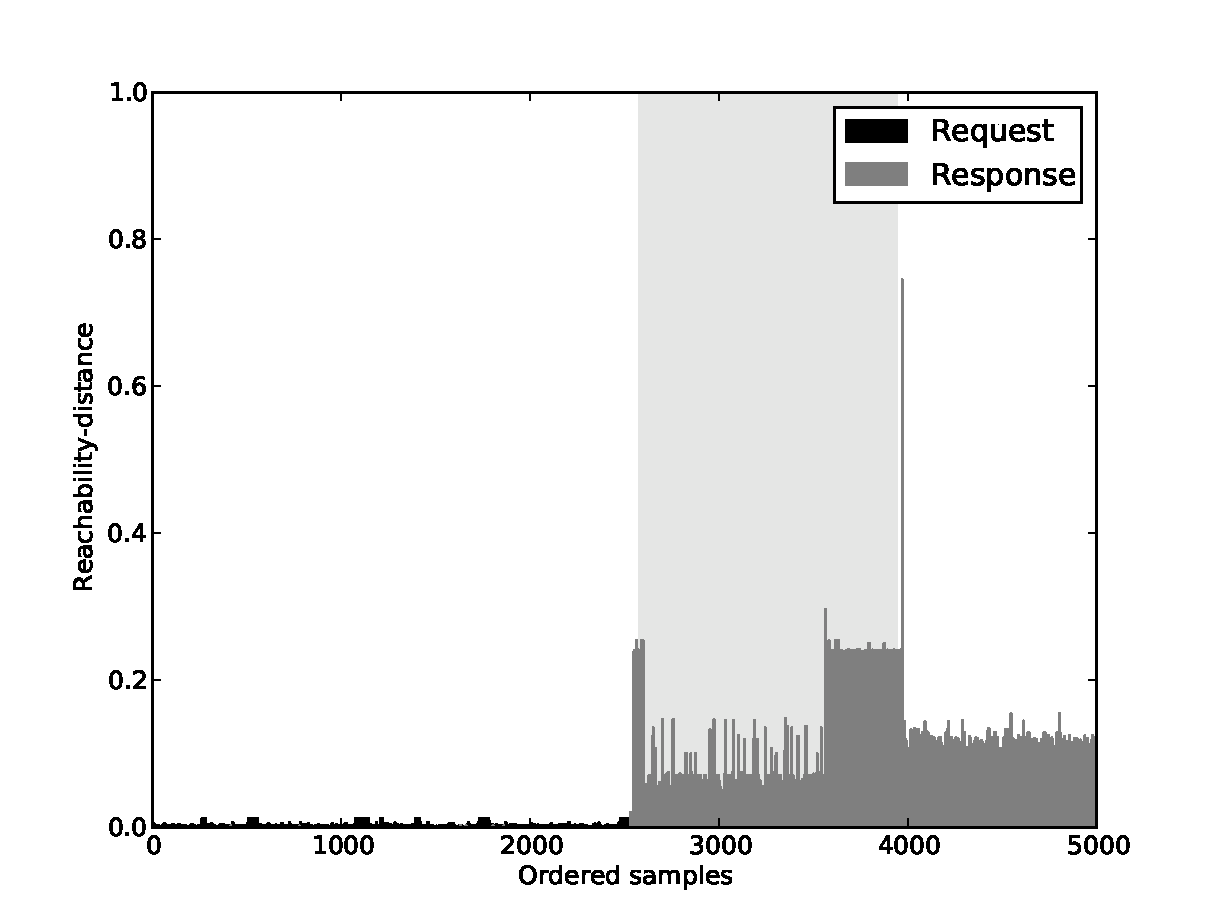
\includegraphics[height=4.5cm]{img/hierextr.pdf}
            \end{column}
        \end{columns}
    \end{frame}
    \begin{frame}
        \frametitle{K: Hitta meddelandetyper -- Klustring (forts.)}
        Egenskaper: Vektor $\{f_1, f_2, ..., f_n\}$
        \begin{itemize}
            \item $n$: Meddelandets längd
            \item $f_i$: Sannolikhet för att bytevärdet på position $i$ i
                meddelandet är det värdet som det är.
        \end{itemize}
        \vskip20pt
        Problem: Hög dimensionalitet \\
        \begin{itemize}
            \item Skillnader mellan data blir mindre signifikant då
                dimensionaliteten ökar
        \end{itemize}
        Lösning: \textbf{PCA}, \scriptsize{\underline{P}rincipal
            \underline{C}omponent \underline{A}nalysis} \\
        PCA:
        \begin{itemize}
            \item Projicerar ner våra egenskaper till en lägre dimensionalitet
                där en bestämd mängd av variansen bibehålls
            \item I vårt fall: bibehåller 80\% av variansen
        \end{itemize}
    \end{frame}
    \begin{frame}
        \frametitle{K: Hitta meddelandetyper -- Förfining}
        \begin{itemize}
            \item \emph{Typ-bytes}: Bytes som bestämmer ett meddelandes typ \\
                \begin{itemize}
                    \item Exempel: SMB, byte som bestämmer typ
                    \item Exempel: DNS, bit som bestämmer query eller response
                \end{itemize}
            \item Antagande: Om det finns typ-bytes så kommer de oftast ha
                samma värde inom kluster \\
                \begin{itemize}
                    \item Eftersom paket inom kluster är mycket lika varandra,
                        och därför sannolikt är av samma typ
                \end{itemize}
            \item \emph{Completeness}: Hög om många datapunkter av en viss
                sann typ ligger inom samma kluster
        \end{itemize}
        \vskip20pt
        \textbf{Metod}: För varje byte-position, dela upp alla meddelanden
        efter de värden som byten antar. Har indelningen hög completeness mot
        OPTICS-klustringen: \underline{möjlig typ-byte}
    \end{frame}

    % Fält
    \begin{frame}
        \frametitle{F: Protokollens fält}
        \begin{itemize}
            \item Lagrar data som är intressant för protokollet
            \item Ligger ofta justerade efter 1, 2 eller 4 bytes
                \begin{itemize}
                    \item Prestandavinst om de ligger alignade.
                \end{itemize}
            \item Fälttyper vi observerat:
                \begin{itemize}
                    \item Konstanta fält
                    \item Flaggfält
                    \item Uniformt fördelade fält
                    \item Nummerfält
                    \item Inkrementella fält
                    \item Längdfält
                \end{itemize}
            \item Många fälttyper har speciell fördelning av bytevärden
                \begin{itemize}
                    \item Fördelning i enbytes-fallet: antal gånger ett visst
                        bytevärde mellan 0 och 255 uppträder på en viss position
                        i meddelandet.
                \end{itemize}
        \end{itemize}
    \end{frame}

    % Något om hur vi kör vår klassificering

    \begin{frame}
        \frametitle{F: Konstanta fält}
        \begin{columns}[t]
            \begin{column}[T]{6cm}
                \begin{itemize}
                    \item Antar bara ett värde för alla meddelanden
                    \item Kan vara konstant globalt, inom ström, inom
                        anslutning eller inom typ
                    \item Lätt att klassificera
                \end{itemize}
                Exempel:
                \begin{itemize}
                    \item Reserverade fält, ofta nollor
                    \item Fält som i övrigt är specificerade som konstanta
                        enligt protokollspecifikationen
                    \item Värden som alltid är samma inom vår dump
                \end{itemize}
            \end{column}
            \begin{column}[T]{6cm}
                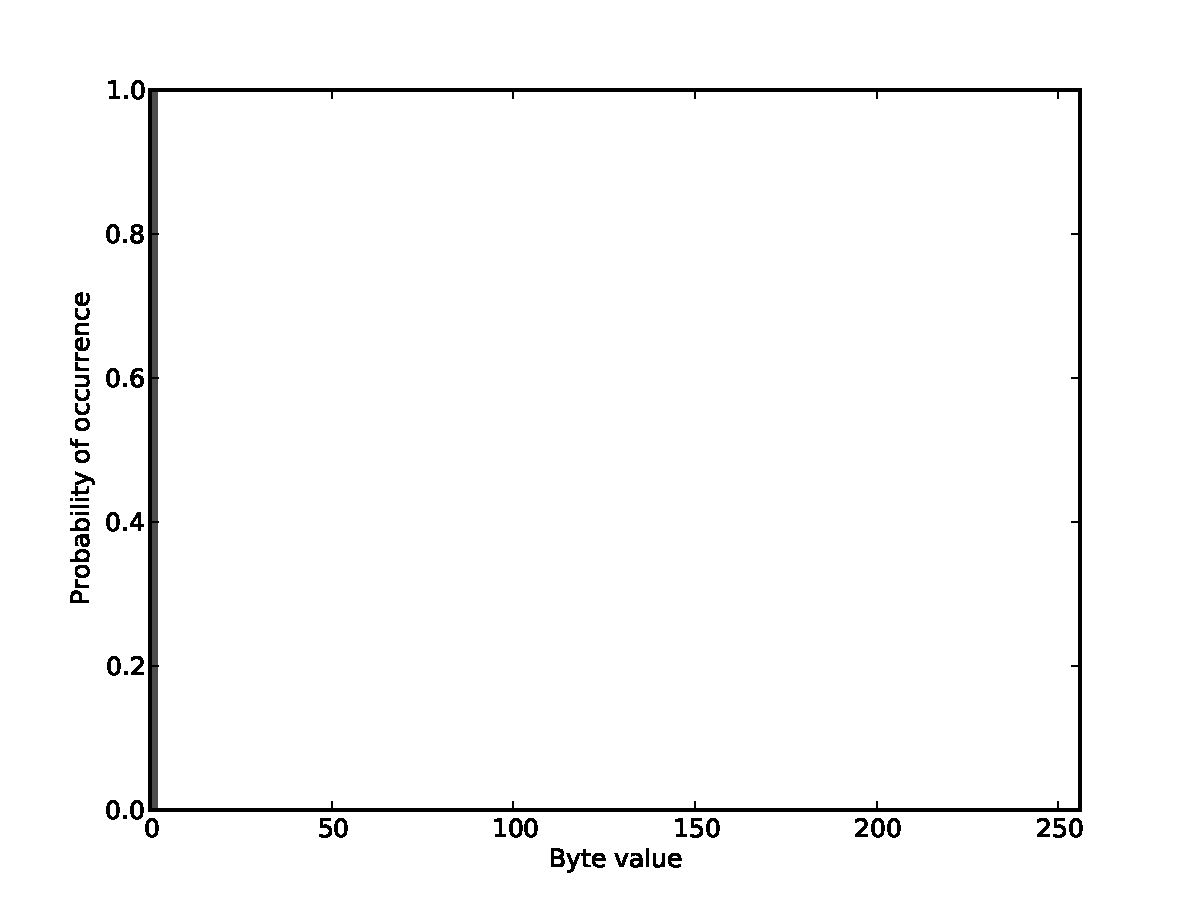
\includegraphics[height=5cm]{img/const_one.pdf}
            \end{column}
        \end{columns}
    \end{frame}
    \begin{frame}
        \frametitle{F: Flaggfält}
        \begin{columns}[t]
            \begin{column}[T]{6cm}
                \begin{itemize}
                    \item Antar fåtal värden för alla meddelanden
                    \item Klassificerar som flaggfält om fält antar minst
                        två värden men mindre värden än en övre gräns
                \end{itemize}
                Exempel:
                \begin{itemize}
                    \item Request/response-flagga
                    \item Bit som indikerar om fel inträffat
                    % mer?
                \end{itemize}
                Bild: Flaggbyte i DNS. 0 = request, 128 = response
            \end{column}
            \begin{column}[T]{6cm}
                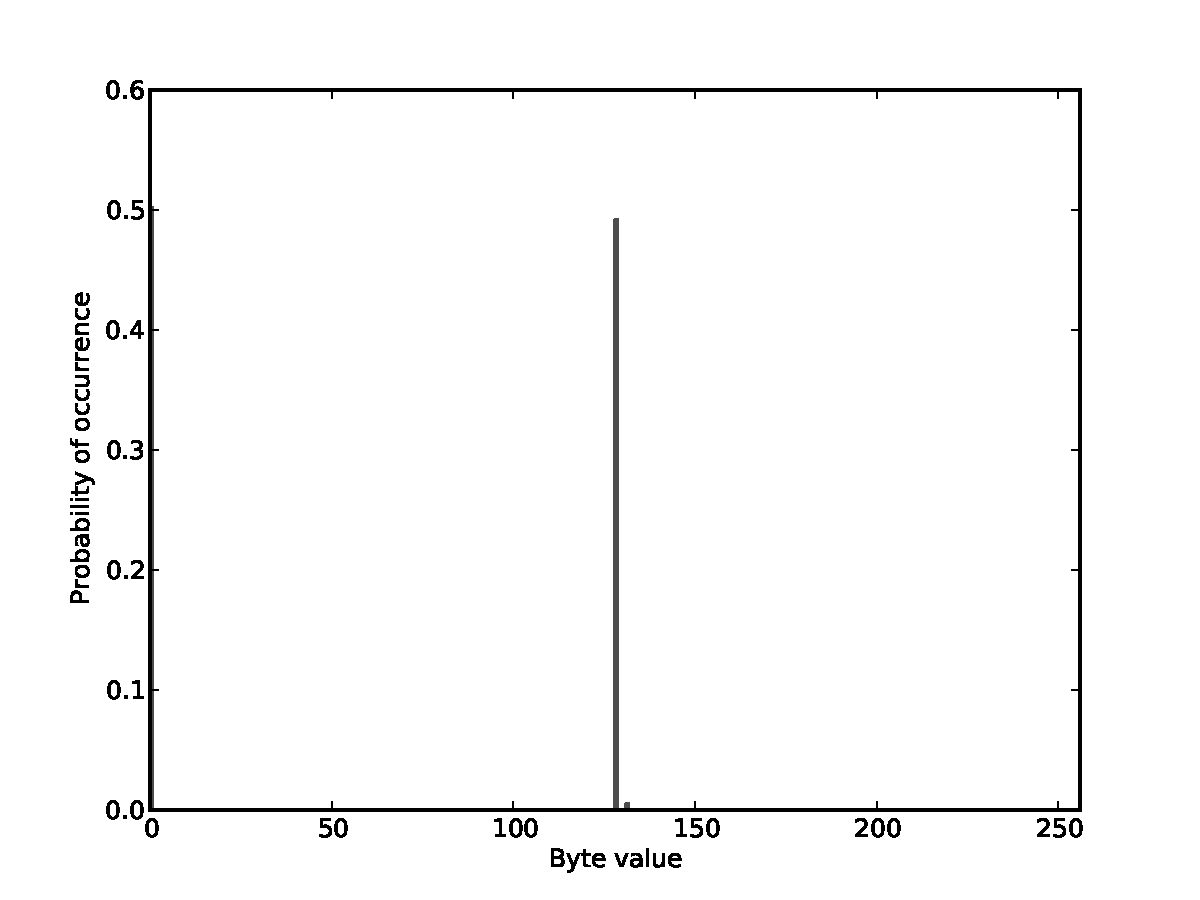
\includegraphics[height=5cm]{img/flag.pdf}
            \end{column}
        \end{columns}
    \end{frame}
    \begin{frame}
        \frametitle{F: Uniformt fördelade fält}
        \begin{columns}[t]
            \begin{column}[T]{6cm}
                \begin{itemize}
                    \item Uniform fördelning: Vanlig för slumptal
                    \item Vanlig för genererade värden så som ID:n eller nonces
                    \item Klassificerar som uniformt om avstånd till 
                        rektangulär- fördelning är låg
                        \begin{itemize}
                            \item Linjen ligger på $\frac{1}{2^{8 \cdot antal bytes}}$
                        \end{itemize}
                \end{itemize}
                Bild: Transaction ID i DNS
            \end{column}
            \begin{column}[T]{6cm}
                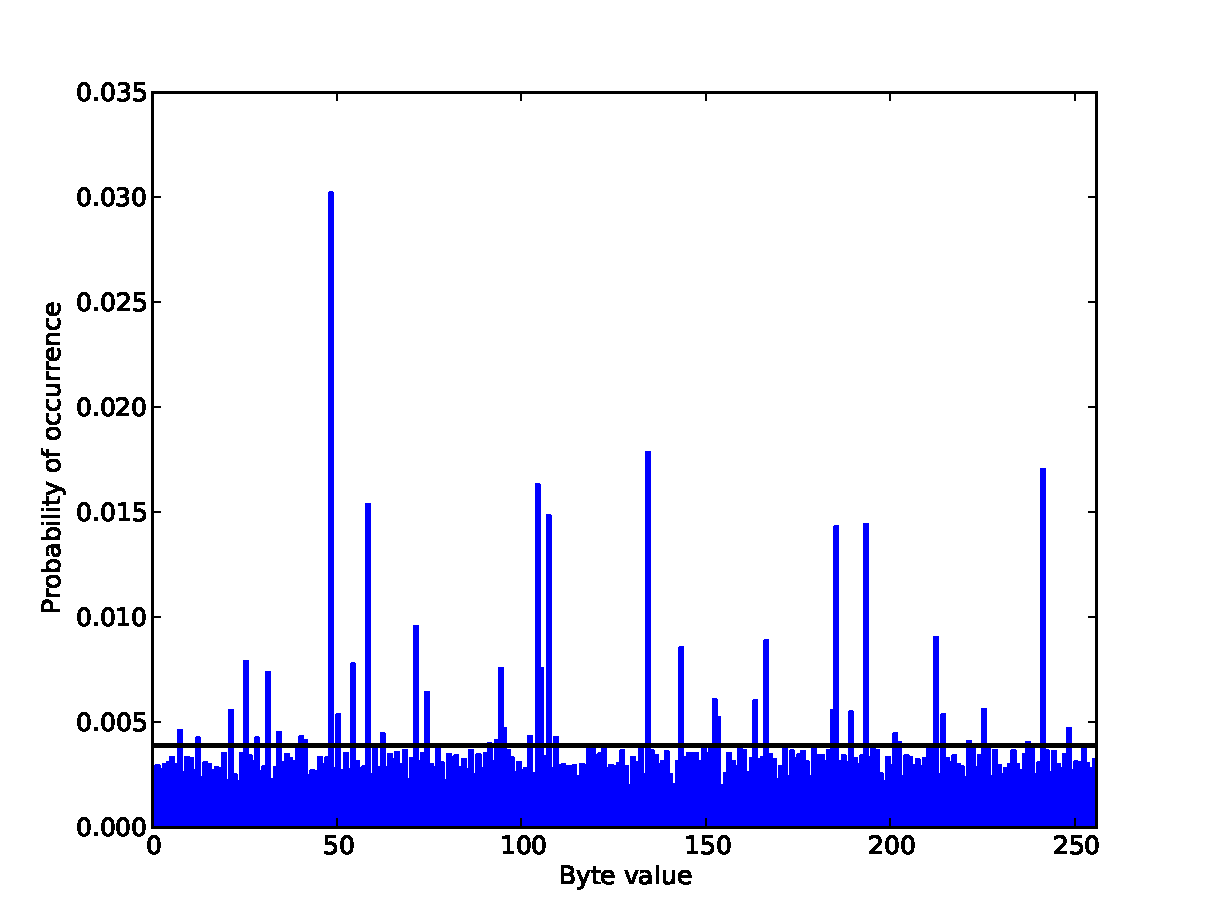
\includegraphics[height=5cm]{img/uniform.pdf}
            \end{column}
        \end{columns}
    \end{frame}
    \begin{frame}
        \frametitle{F: Nummerfält}
        \begin{columns}[t]
            \begin{column}[T]{6cm}
                \begin{itemize}
                    \item Fält som innehåller nummer, t.ex. antal
                    \item Observation: Normalfördelade
                    \item Klassificerar som nummerfält om vi kan få avståndet
                        till någon normalfördelningskurva att understiga ett
                        visst värde
                \end{itemize}
            \end{column}
            \begin{column}[T]{6cm}
                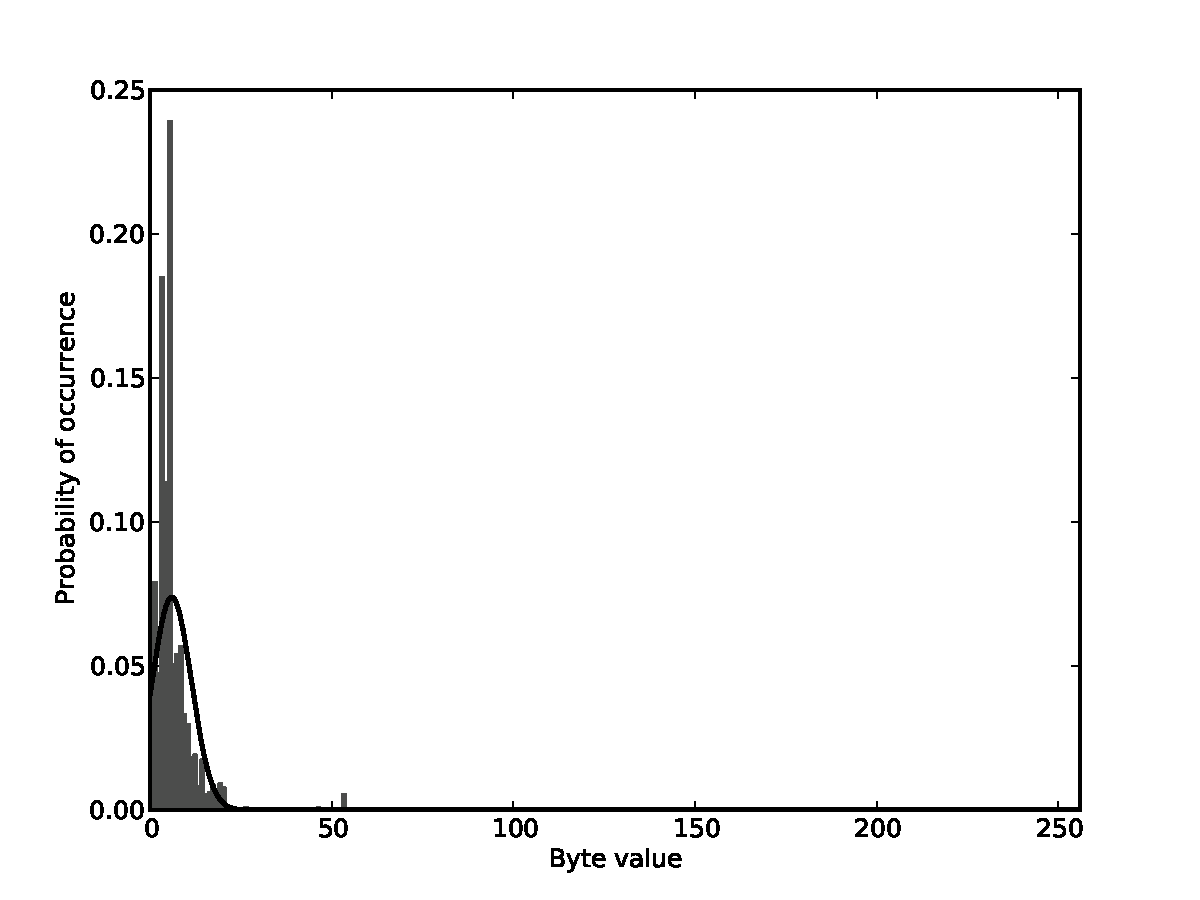
\includegraphics[height=5cm]{img/number.pdf}
            \end{column}
        \end{columns}
    \end{frame}
    \begin{frame}
        \frametitle{F: Inkrementella fält}
        \begin{itemize}
            \item Bytevärdesdistribution är ointressant
                \begin{itemize}
                    \item Kollar följd av värden istället för distribution
                \end{itemize}
            \item Kan bara upptäckas inom ström eller anslutning
                \begin{itemize}
                    \item Globalt inkrementellt är osannolikt, även för t.ex. timestamps (olika klockor)
                \end{itemize}
            \item Exempel: Sekvensnummer, räknare, tid
            \item Klassificerar som inkrementellt fält om dess värde
                oftast\footnote{Efter 255 kommer 0} är ökande genom
                ström/anslutning
        \end{itemize}
    \end{frame}
    \begin{frame}
        \frametitle{F: Längdfält}
        \begin{columns}[t]
            \begin{column}[T]{6cm}
                \begin{itemize}
                    \item Bestämmer längd på något fält inom meddelande
                    \item Observation: Värde i längdfält är proportionellt
                        mot meddelandets längd
                    \item Problem: Fragmentering
                    \item Lösning: RANSAC
                \end{itemize}
                Inte bara längd för hela meddelandet, utan även längd på delar
                av meddelandet, t.ex. payload utan header.\\
                \vskip20pt
                Bild 1: RANSAC vs Ordinary Least Squares. Hanterar outliers.\\
                \vskip20pt
                Bild 2: Wordcount i SMB. Visar på hur vi kan hitta linjära
                samband trots fragmentering etc.
            \end{column}
            \begin{column}[T]{6cm}
                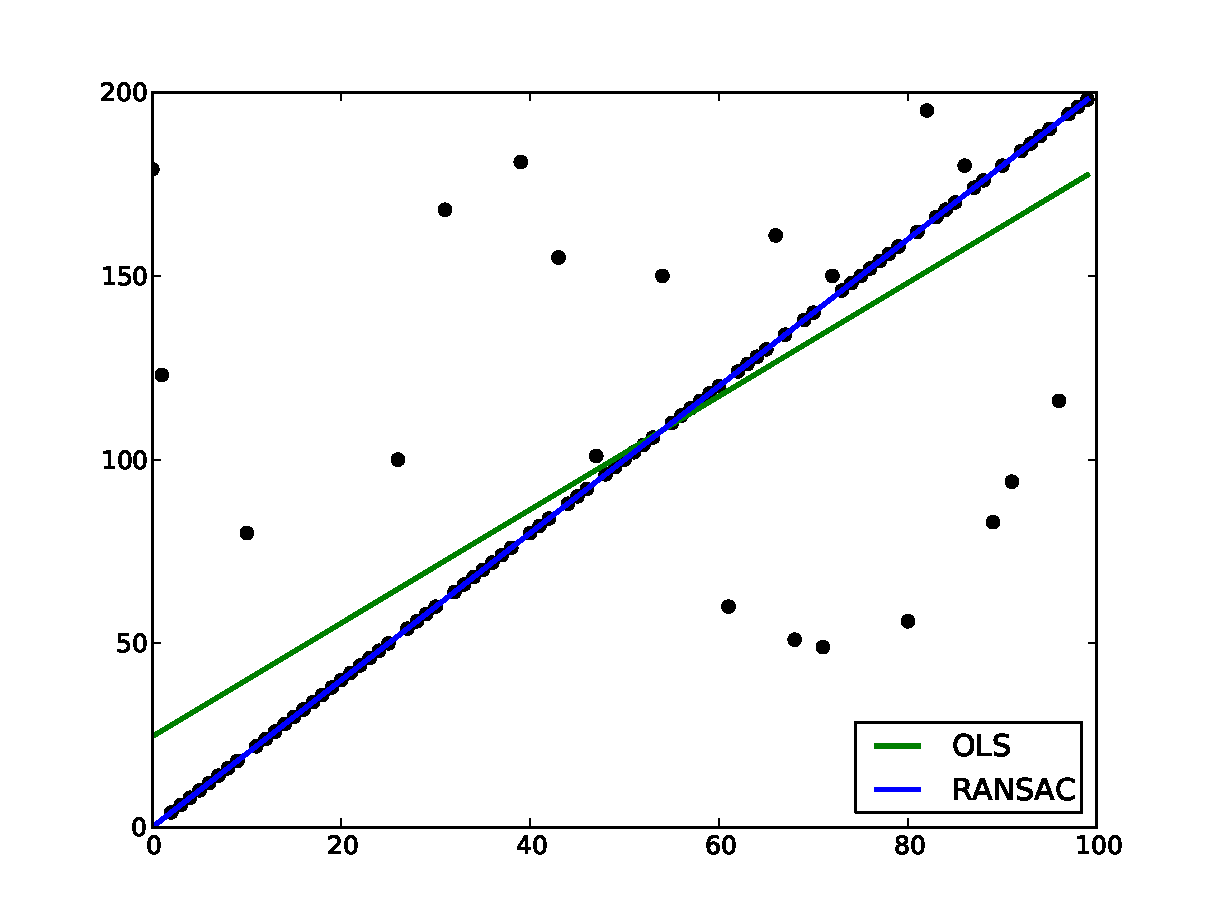
\includegraphics[height=4cm]{img/ransac.pdf}\\
                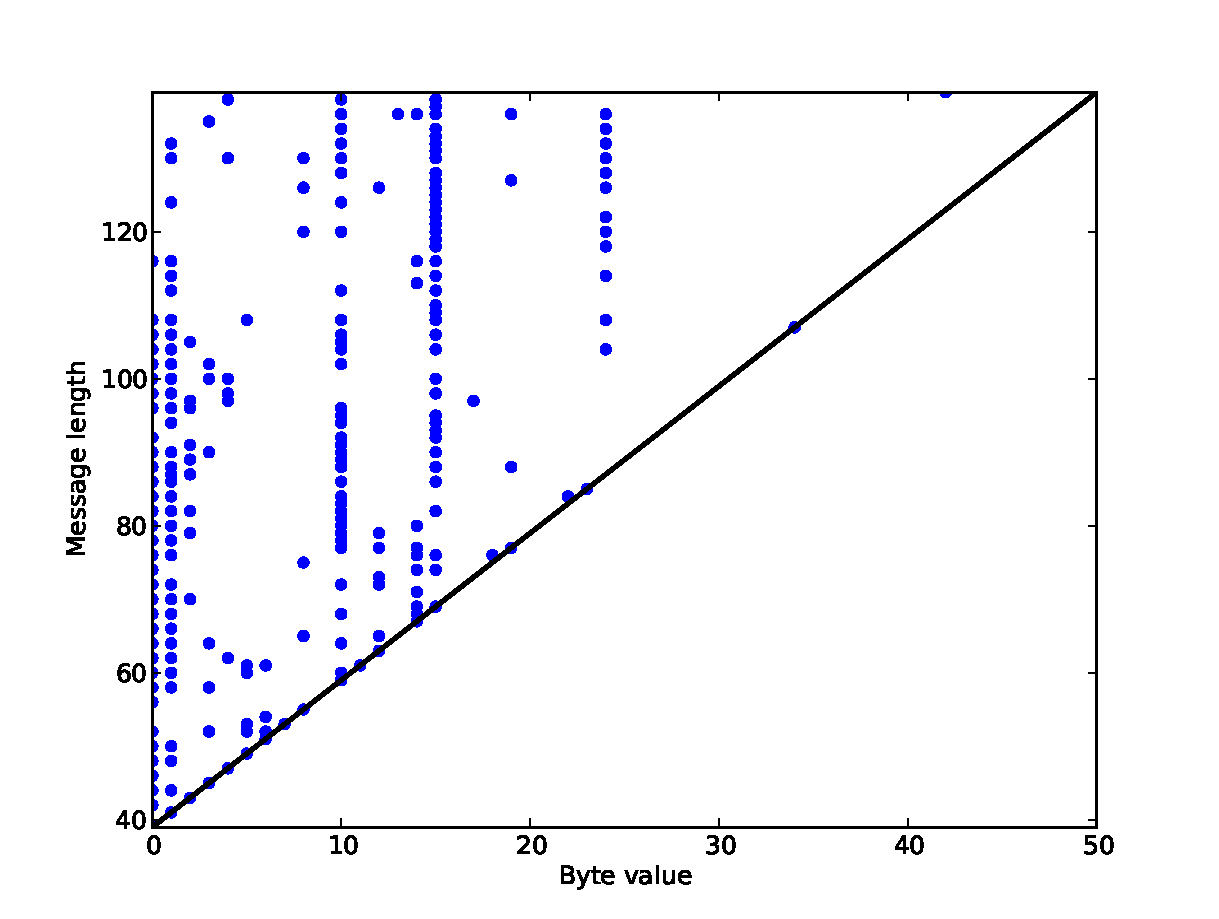
\includegraphics[height=4cm]{img/length.pdf}
            \end{column}
        \end{columns}
    \end{frame}

    % Tillstånd
    \begin{frame}
        \frametitle{K: Protokolls tillstånd}
        \begin{itemize}
            \item Protokoll modelleras ofta efter \emph{tillståndsdiagram}
            \item Vet vilka typer som finns och i vilken ordning de skickats
            \item Kan delvis återskapa tillståndsdiagrammet
            \item Att återskapa tillståndsdiagrammet för alla tillstånd är
                oftast för rörigt. Nöjer oss med protokollets initiering.
                \begin{itemize}
                    \item Kan även vara intressant under andra tillstånd så
                        som filöverföring etc.
                \end{itemize}
        \end{itemize}
        Prick: Tillstånd innan någon kommunikation har skett\\
        Dubbelcirkel: Sluttillstånd
        \vskip10pt
        Bild 1: DNS. Pilar till 0: Query. Pilar till 1: Response
        \vskip10pt
        Bild 2: SMB. Handskakning
        \begin{columns}[t]
            \begin{column}[T]{5cm}
                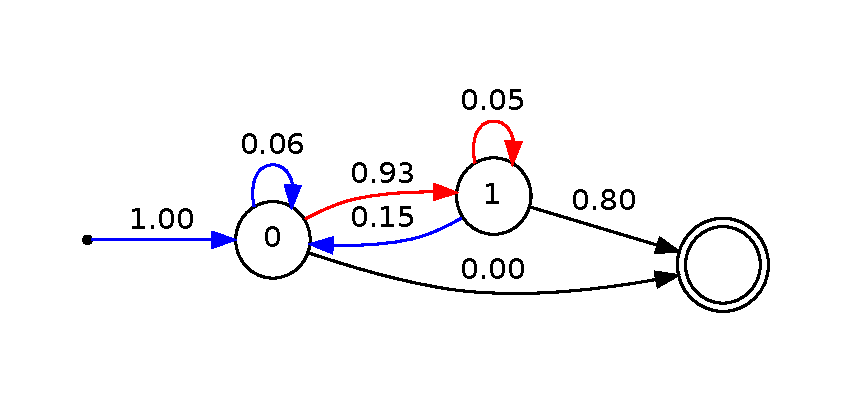
\includegraphics[height=3cm]{img/dnsstate.pdf}
            \end{column}
            \begin{column}[T]{6cm}
                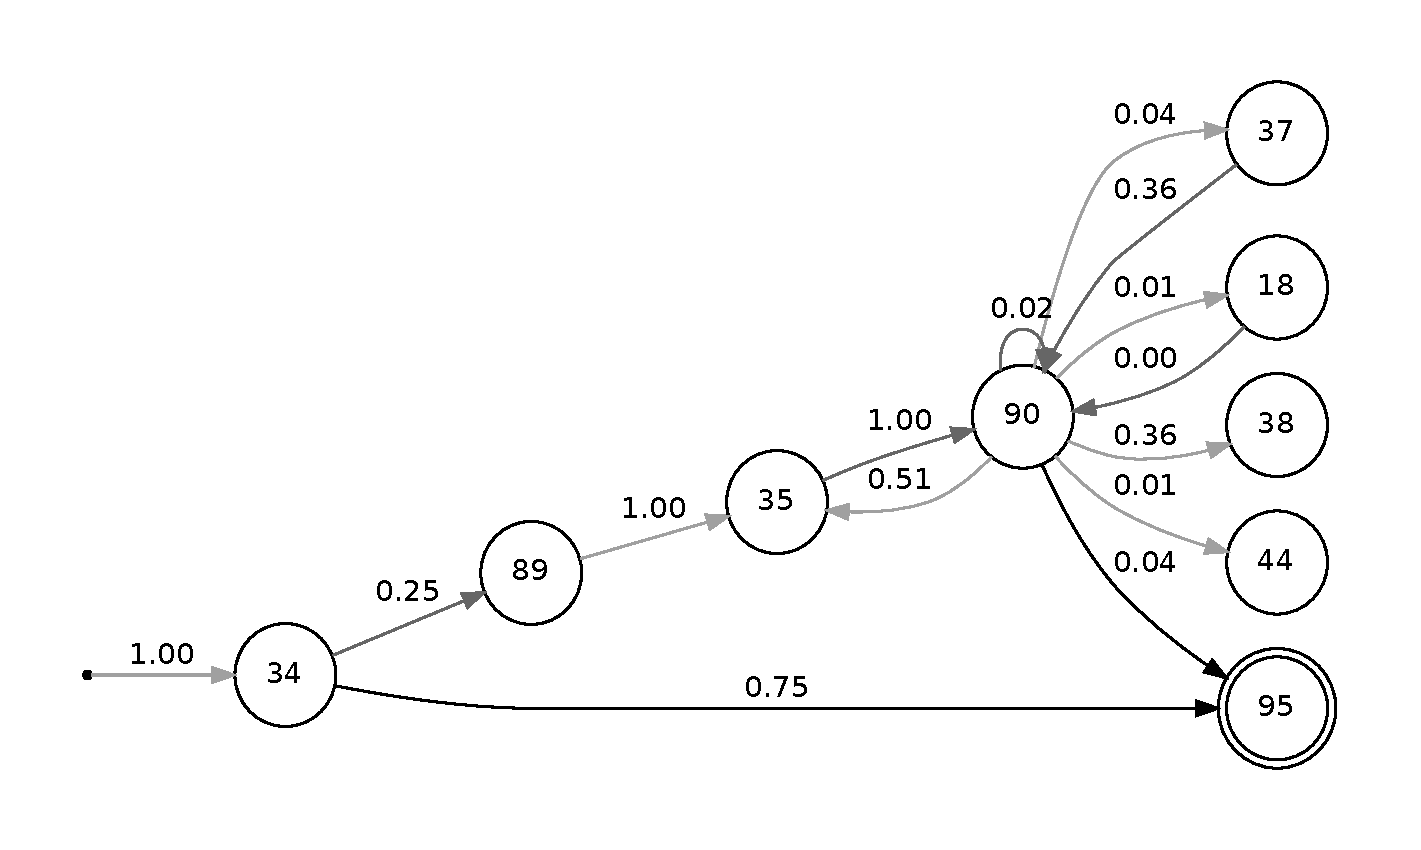
\includegraphics[height=3.5cm]{img/smbstate.pdf}
            \end{column}
        \end{columns}

    \end{frame}

    % Resultat
    \begin{frame}
        \frametitle{K: Resultat -- Klustring}
        Resultat efter OPTICS:
        \begin{table}[h]
            \centering
            \scriptsize{
                \begin{tabular}{| l | r | r | r | r | r |}
                    \hline
                    \textbf{Protokoll}&\textbf{Completeness}&\textbf{Homogenity}&\textbf{V-measure} \\ \hline
                    DNS & 0.1982 & 0.9550 & 0.3282 \\ \hline
                    SMB & 0.8480 & 0.8632 & 0.8555 \\ \hline
                    TFTP & 0.3015 & 0.9449 & 0.4571 \\ \hline
                    RTP & 0.0000 & 1.0000 & 0.0000 \\ \hline
                    DHCP & 0.3492 & 0.1224 & 0.1813 \\ \hline
                \end{tabular}
            }
        \end{table}
        Resultat efter förfining:
        \begin{table}[h]
            \centering
            \scriptsize{
                \begin{tabular}{| l | r | r | r | r | r |}
                    \hline
                    \textbf{Protokoll}&\textbf{Completeness}&\textbf{Homogenity}&\textbf{V-measure} \\ \hline
                    DNS & 0.9534 & 0.9999 & 0.9761 \\ \hline
                    SMB & 0.9914 & 0.9880 & 0.9897 \\ \hline
                    TFTP & 1.0000 & 1.0000 & 1.0000 \\ \hline
                    RTP & 0.0000 & 1.0000 & 0.0000 \\ \hline
                    DHCP & 1.0000 & 0.4428 & 0.6138 \\ \hline
                \end{tabular}
            }
        \end{table}
        Förklaring:
        \begin{itemize}
            \item Completeness: Hög när stor del av viss sann typ ligger i
                samma kluster
            \item Homogenity: Hög när kluster till stor del endast innehåller
                viss typ
            \item V-measure: Kombination av de båda
        \end{itemize}
    \end{frame}
    \begin{frame}
        \frametitle{K: Resultat -- Fält}
        \begin{table}[h]
            \scriptsize{
                \begin{tabular}{| l | r | r | r |}
                    \hline
                    \textbf{Protokoll}&\textbf{\# Korrekta Bitar}&\textbf{\# Bitar Totalt}&\textbf{Riktighet (\%)} \\ \hline
                    DNS & 37 & 96 & 38.5 \\ \hline
                    SMB & 112 & 288 & 38.9 \\ \hline
                    TFTP & 0 & 16 & 0.0 \\ \hline
                    RTP & 40 & 96 & 41.7 \\ \hline
                    DHCP & 64 & 1888 & 3.4 \\ \hline
                \end{tabular}
            }
        \end{table}
        Förklara varför vi aldrig kan få perfekt resultat.

        Exempel: DNS
        \begin{columns}[t]
            \begin{column}[T]{5cm}
                \begin{bytefield}[bitwidth=0.3cm]{16}
                    \bitheader{0, 16}\\
                    \wordbox{1}{U}\\
                    \bitbox{1}{F}
                    \bitbox{4}{F}
                    \bitbox{1}{F}
                    \bitbox{1}{F}
                    \bitbox{1}{F}
                    \bitbox{1}{F}
                    \bitbox{3}{C}
                    \bitbox{4}{F}\\
                    \wordbox{1}{N}\\
                    \wordbox{1}{N}\\
                    \wordbox{1}{N}\\
                    \wordbox{1}{N}
                \end{bytefield}
            \end{column}
            \begin{column}[T]{5cm}
                \begin{bytefield}[bitwidth=0.3cm]{16}
                    \bitheader{0, 16}\\
                    \wordbox{1}{U}\\
                    \bitbox{8}{SC}
                    \bitbox{8}{F}\\
                    \wordbox{1}{C}\\
                    \bitbox{8}{C}
                    \bitbox{8}{N}\\
                    \bitbox{8}{C}
                    \bitbox{8}{N}\\
                    \bitbox{8}{C}
                    \bitbox{8}{UNK}
                \end{bytefield}
            \end{column}
        \end{columns}
    \end{frame}
    % Begränsningar
    \begin{frame}
        \frametitle{K: Begränsningar}
        \begin{itemize}
            \item Textuella protokoll
                \begin{itemize}
                    \item Ej samma krav på ordning av meddelandedata
                    \item Går redan att läsa
                \end{itemize}
            \item Icke-justerad data
                \begin{itemize}
                    \item Finns i t.ex. SMB
                    \item Måste testa med sliding window $\rightarrow$ högre komplexitet
                    \item Ej särskilt vanligt
                \end{itemize}
            \item Bit-precision
                \begin{itemize}
                    \item Analysera på bit-nivå istället för byte-nivå
                    \item Samma komplexitetsproblem som icke-justerad data, då protokoll
                        ej justerar på bit-nivå
                    \item Svårt att hitta mening i enstaka bitar
                \end{itemize}
        \end{itemize}
    \end{frame}

\end{document}
